\subsection{Neural Network Design and Training}
\label{subsec:nntraining}

%\begin{wrapfigure}{r}{0.5\textwidth}
%	\centering
%    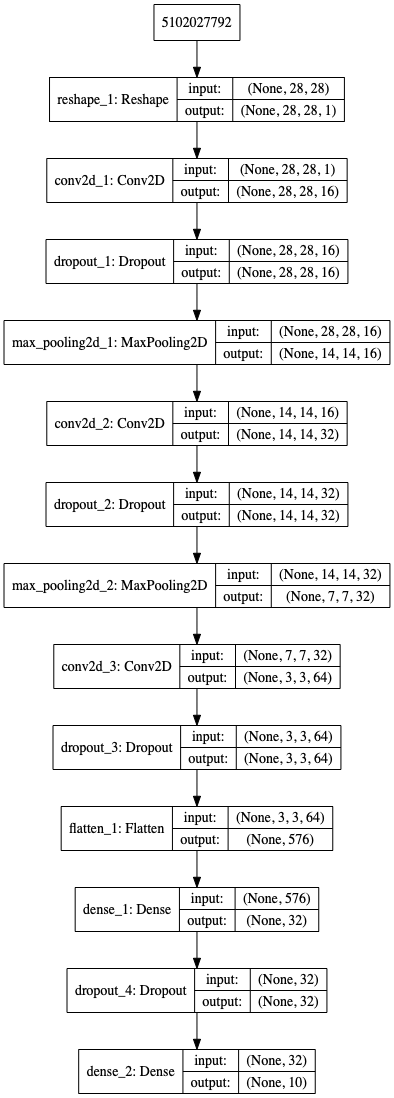
\includegraphics[width=0.35\textwidth]{img/nnlayout}
%	\caption{Network Layers}
%	\label{fig:network-layers}
%\end{wrapfigure}

The network was implemented in PyTorch \cite{Paszke:2019aa} as well as Tensorflow \cite{MartinAbadi:2015aa}. The backend was later exclusively switched to PyTorch (which is also the most common deep learning framework in Science) due to its better support of qunatization. The layers of the network can be seen in Figure~\ref{fig:network-layers}. 
For training of the network the \emph{ADAM} optimization algorithm \cite{Kingma:2014aa} was used to minimize the cross-entropy-loss function which is defined as
\begin{equation}
    J = - y  \log(h) + (1-y)  \log(1-h)
\end{equation}
For controlling the ADAM algorithm the recommended values, listed in Table~\ref{tab:train-params}, by \cite{Kingma:2014aa} was used.
\begin{table}[ht]
	\centering
    \caption{Network Training Parameters}
    \begin{tabular}{cc}
        \toprule
            Parameter & Value \\
        \midrule
            $\alpha$   & $0.001$ \\
            $\beta_1$  & $0.9$   \\
            $\beta_2$  & $0.999$  \\          
        \bottomrule
    \end{tabular}
    \label{tab:train-params}
\end{table}


A useful guide for implementing convolutions can be found in \cite{dumoulin2016guide}. The training 
of the network yielded very high accuracy rates - which is typical for the MNIST dataset, which is for
Machine Learning an easy challenge. Even though the network performance could be improved, e.g. by 
hyperparameter tuning the results were acceptable for our case. The progress of the training in terms
of accuracy and loss can be seen in Figure~\ref{fig:network-train-acc} respectively in Figure~\ref{fig:network-train-loss}.
The final output of the network over the training is evaluated in Figure~\ref{fig:network-test-cm} for real
values and in Figure~\ref{fig:network-test-qcm} for fake quantized values.

\begin{figure}[htbp]
\centering
\begin{subfigure}[t]{0.5\textwidth}
	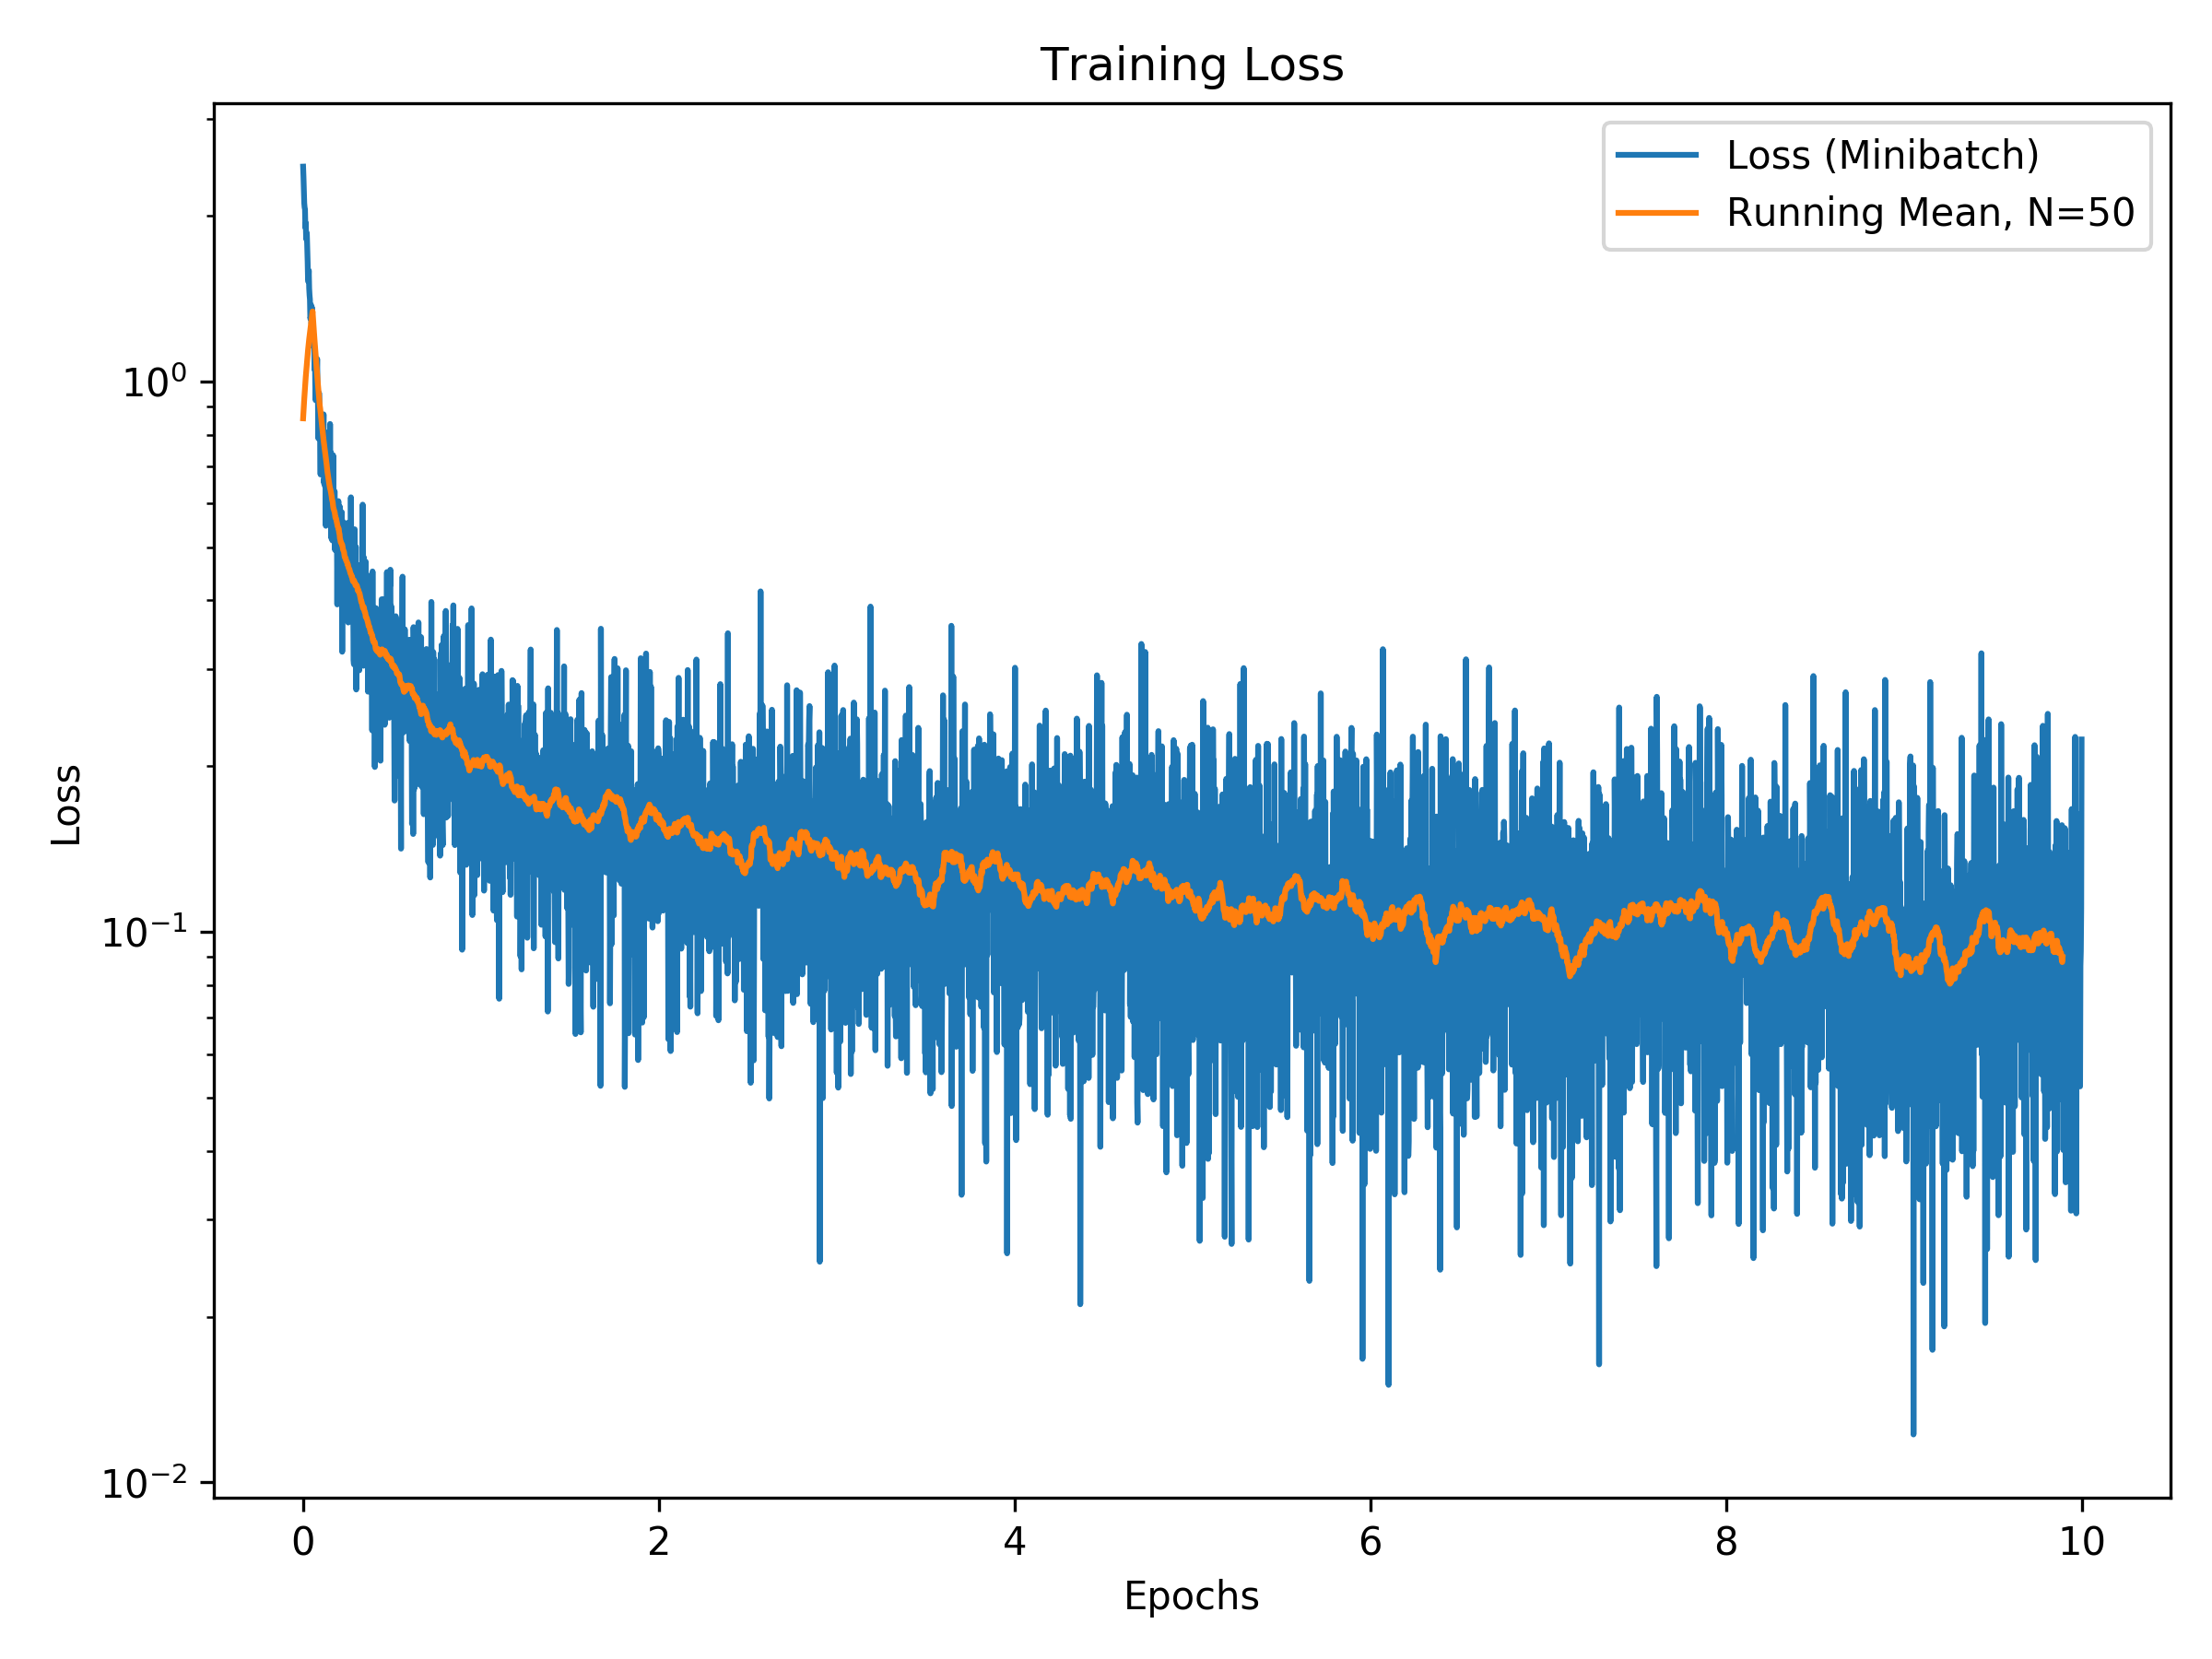
\includegraphics[width=0.8\textwidth]{../../net/images/training_loss}
	\caption{Training Loss}		
	\label{fig:network-train-loss}
\end{subfigure}%
~
\begin{subfigure}[t]{0.5\textwidth}
	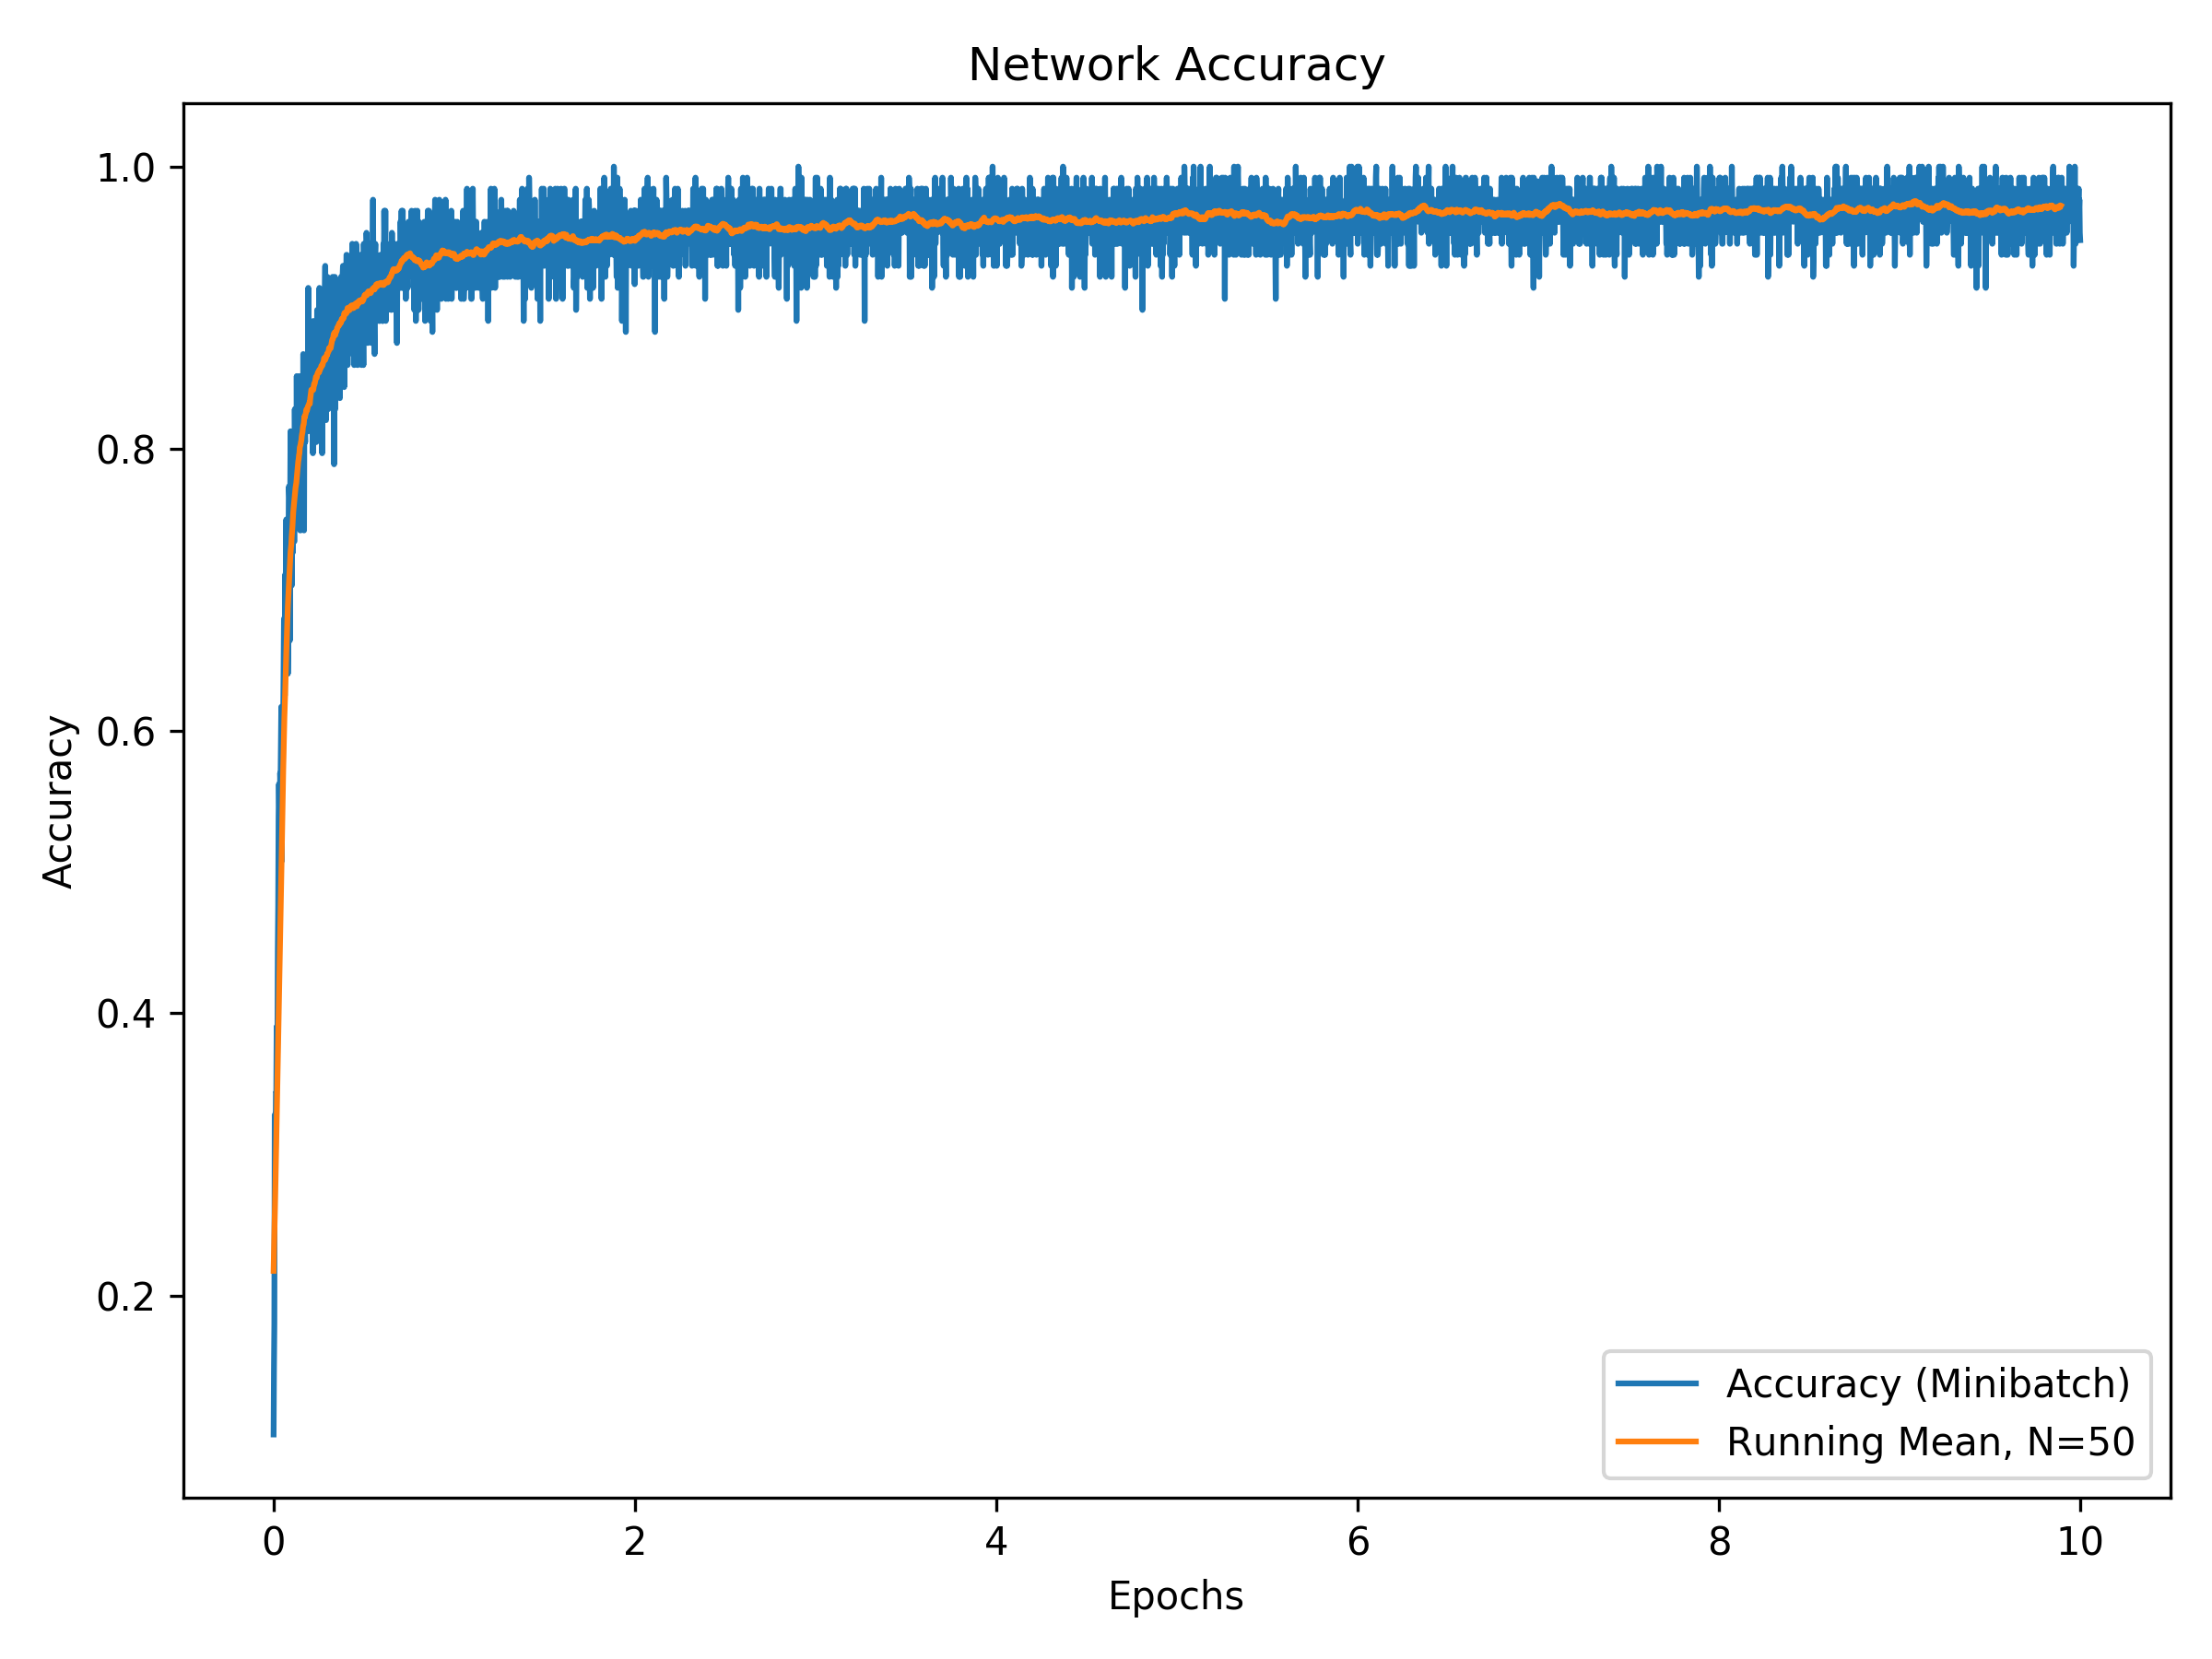
\includegraphics[width=0.8\textwidth]{../../net/images/training_accuracy}
	\caption{Training Accuracy}
	\label{fig:network-train-acc}		
\end{subfigure}
\caption{Network loss and accuracy over the training iterations}
\label{fig:network-training-graphs}
\end{figure}

\begin{figure}
\centering
\begin{subfigure}[t]{0.5\textwidth}
	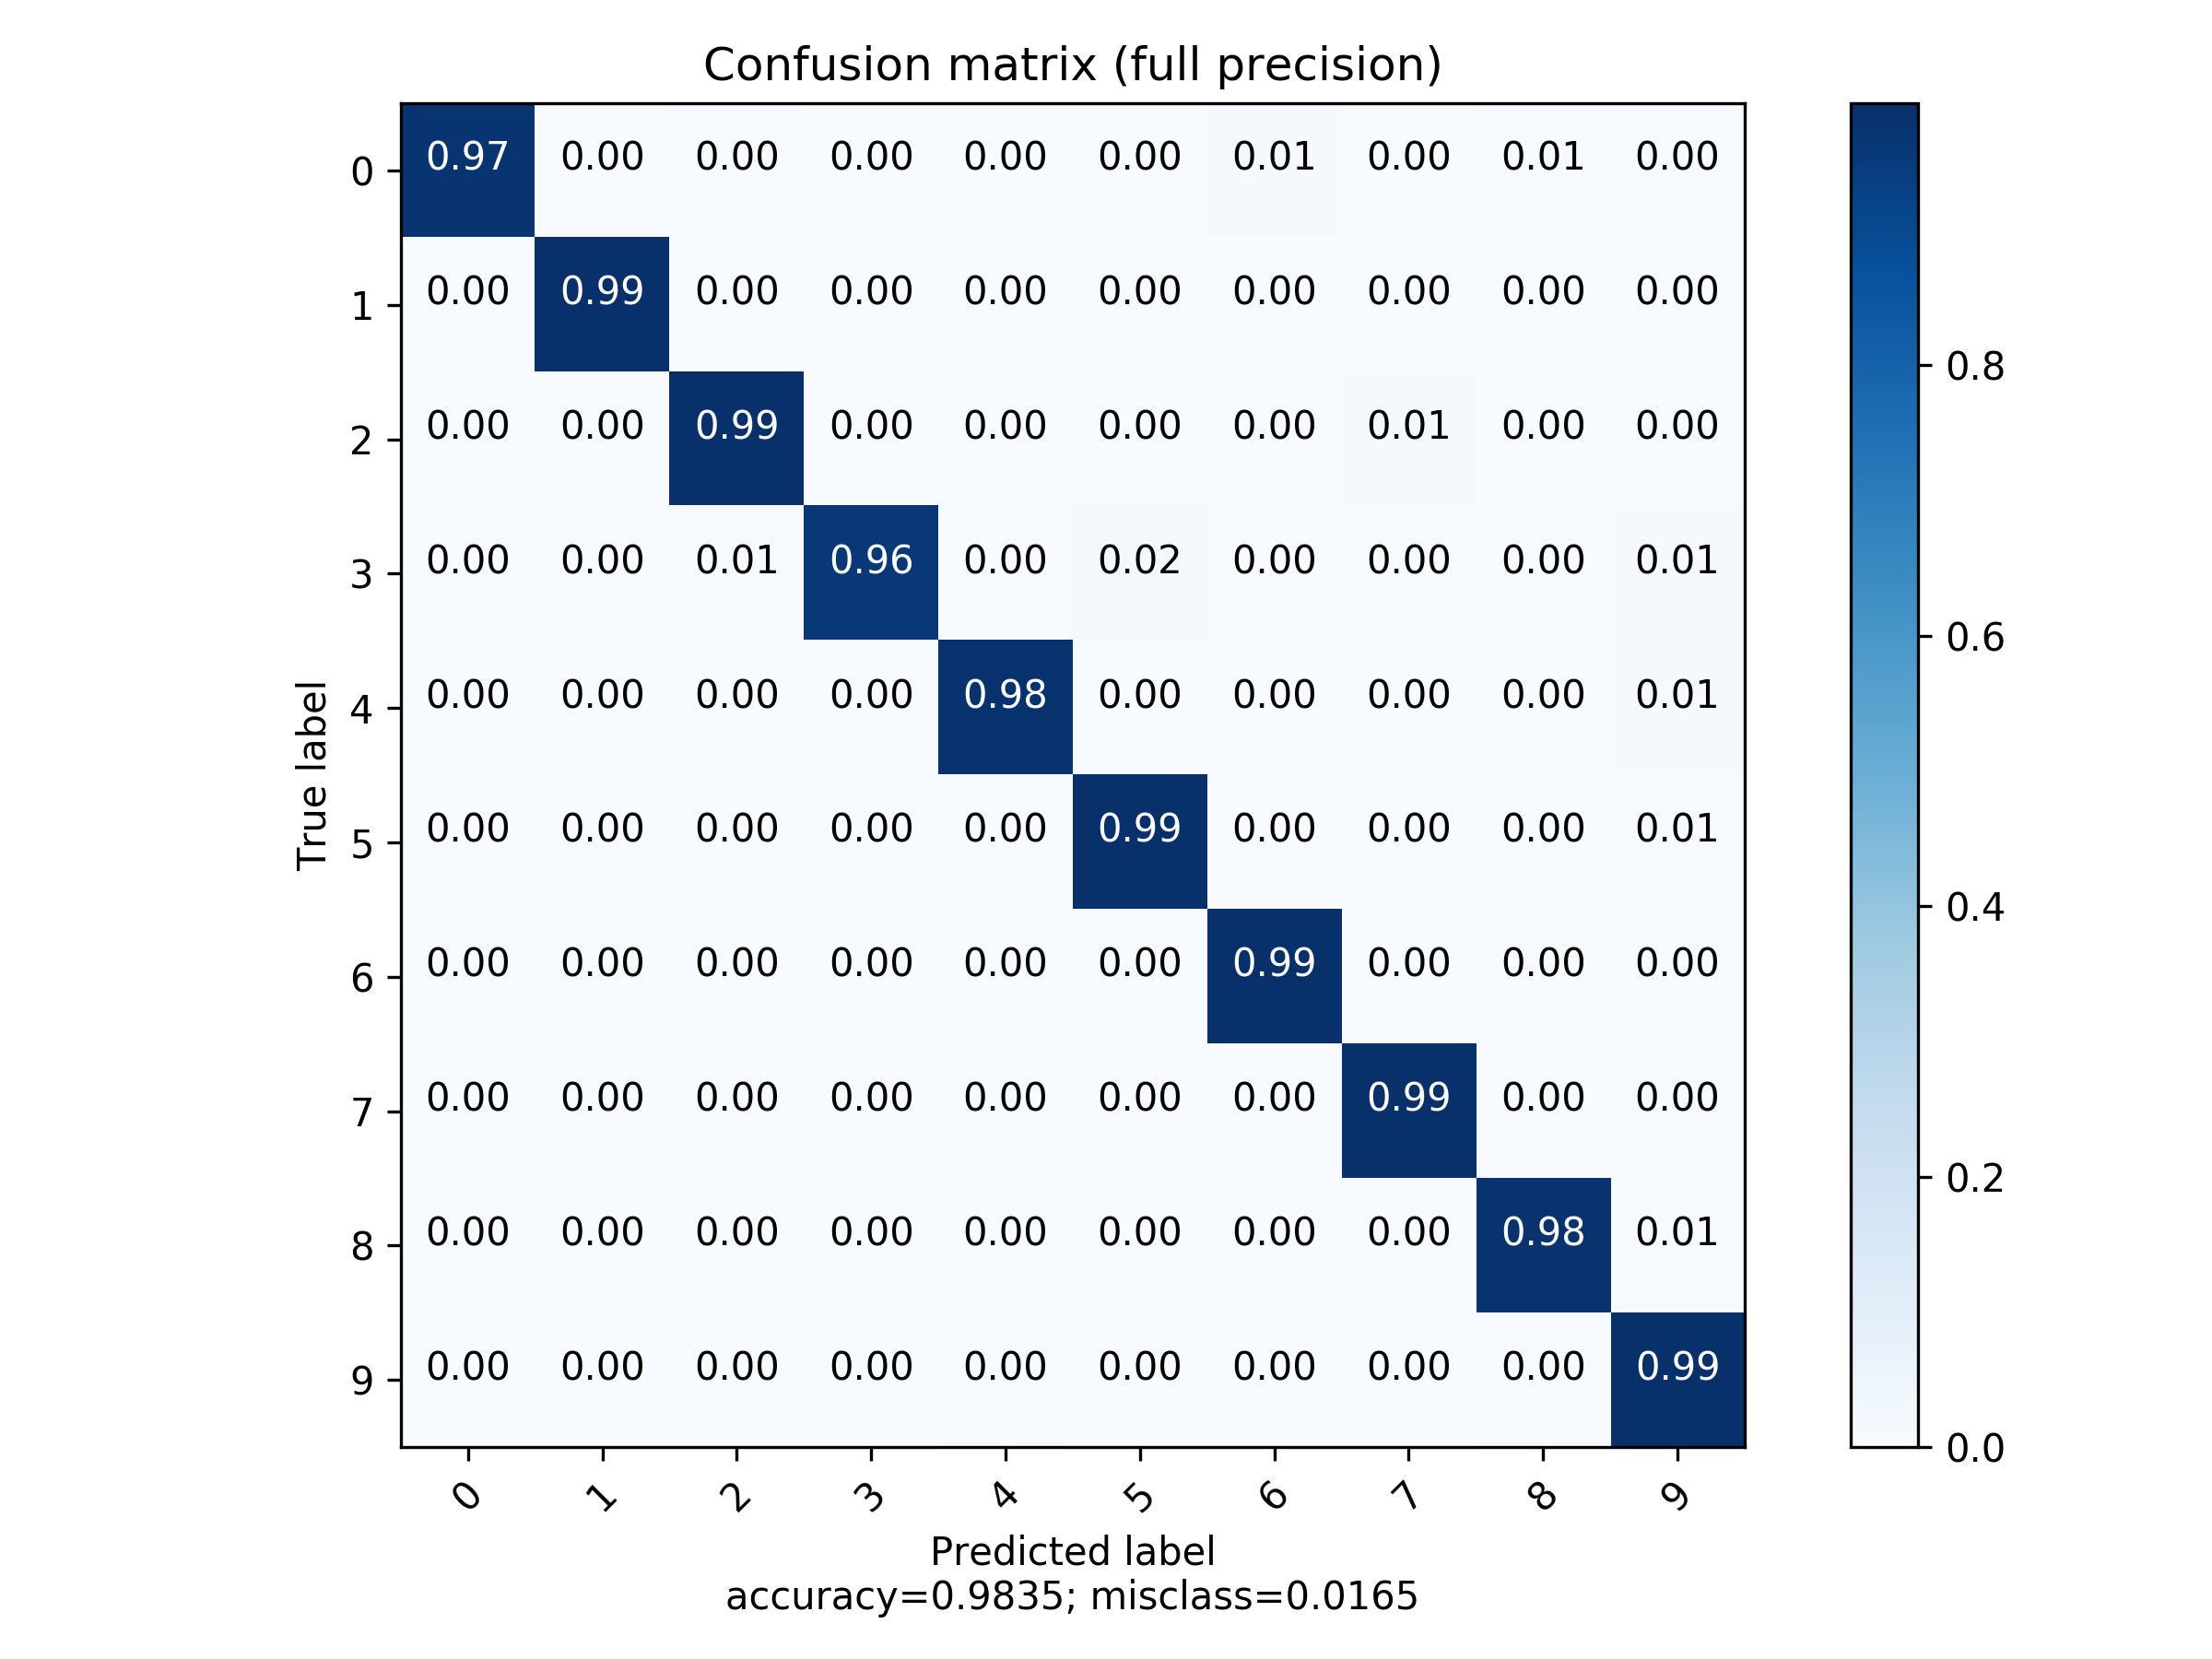
\includegraphics[width=0.9\textwidth]{../../net/images/cm}
	\caption{Floating Point}
	\label{fig:network-test-cm}
\end{subfigure}%
~
\begin{subfigure}[t]{0.5\textwidth}
	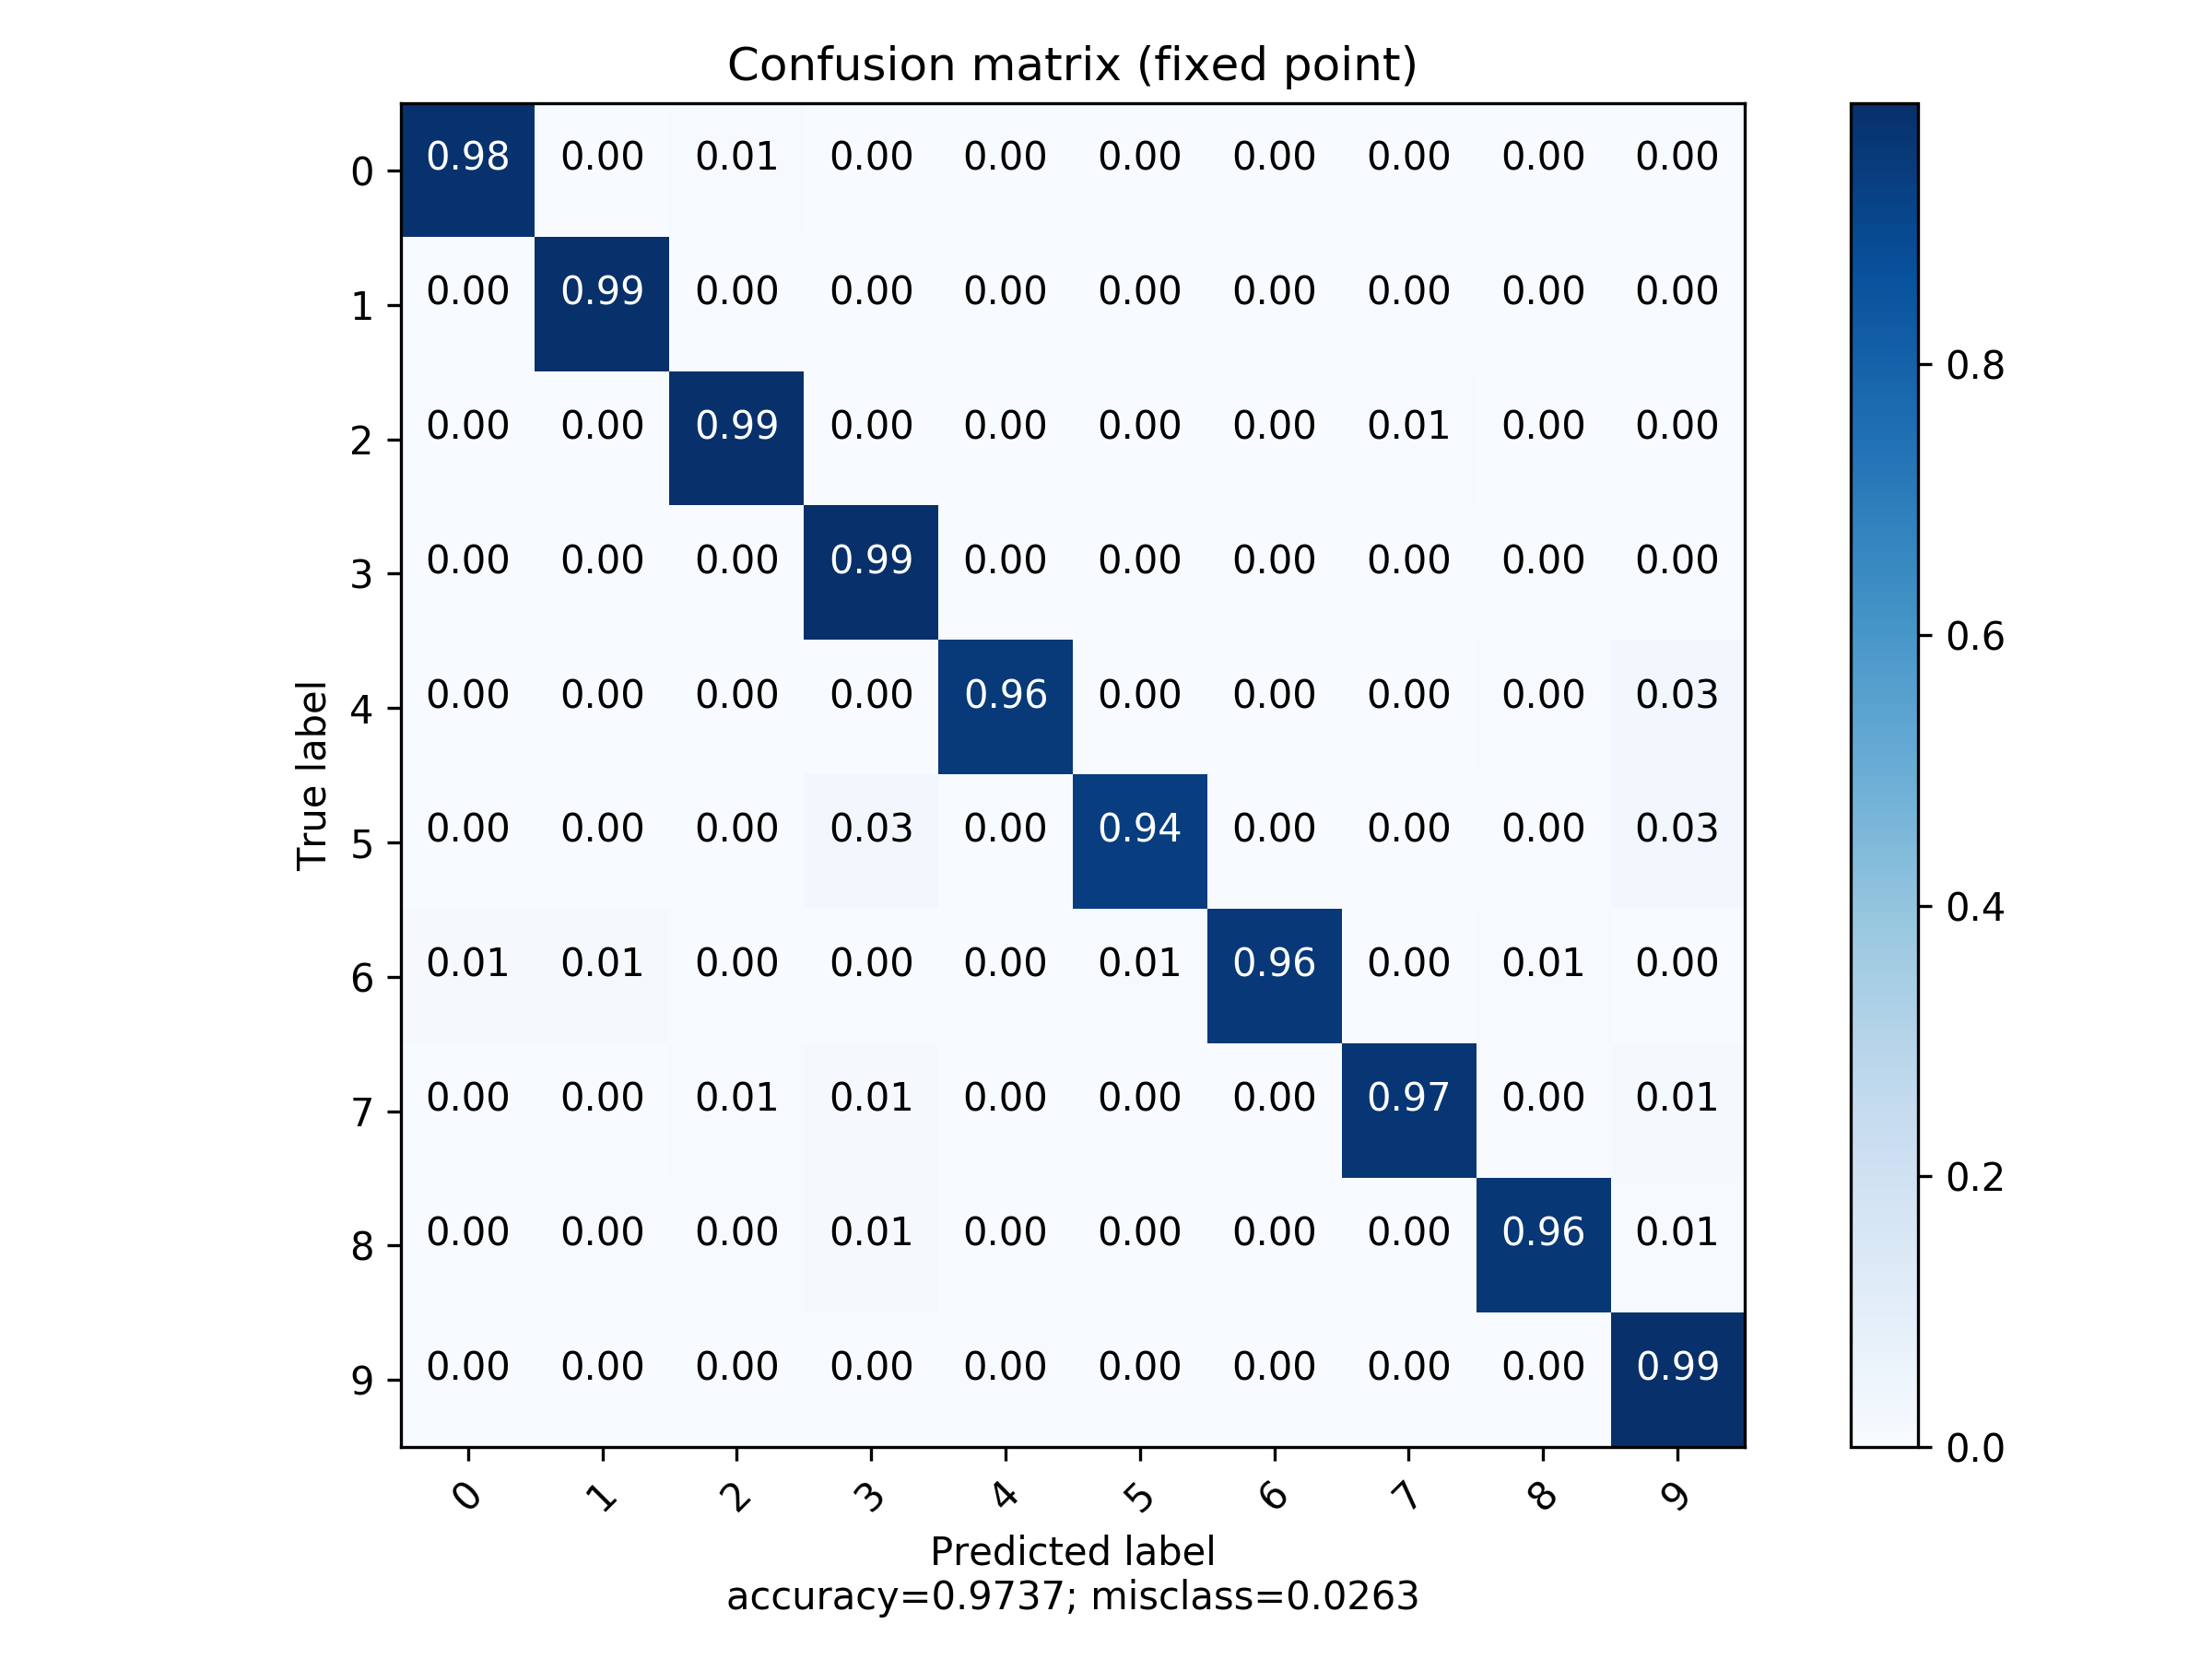
\includegraphics[width=0.9\textwidth]{../../net/images/qcm}
	\caption{Quantized Values}
	\label{fig:network-test-qcm}
\end{subfigure}
\caption{Confusion matrix for the floating point and quantized version of the netowork.}
\label{fig:network-confusion-matrix}
\end{figure}

\subsection{Quantization}

The network is trained and created using 32bit floating point values in Python. Directly porting this all the weights and biases to the FPGA is due to the limited amount of available resources not feasible. The goal is therefore to reduce the amount of required hardware cells by switching from floating point arithmetic to the less expensive integer arithmetic. Then a floating point value $v$ can be approximately represented as 
\begin{equation}
	v \approx Q \cdot 2 ^{-m}
\end{equation}
where $Q$ and $m$ are integers. In our case all input values of the first layer are guaranteed to lie in the interval $[0,1]$ and all layer weights are known from training. It is therefore possible to precompute the expected range where the output values will be. Depending on this range it is then possible to select a suitable bit width for both $Q$ and $m$.

This is a cost-accuracy trade-off where higher bit widths would improve accuracy as well as increase the amount of hardware resources needed.
In \cite{Wu:2018aa} different strategies of choosing bit widhts for $Q$ and $m$ are compared and they observed three main configurations, which are (from simple to advanced):
\begin{enumerate}
	\item Use a $(Q,m)$ configuration for the whole network
	\item Use a $(Q,m)$ configuration for each layer
	\item Use a $(Q,m)$ configuration for each output channel 
\end{enumerate}
In the third configuration the authors could reduce the bit widths the most without sacrificing accuracy this increases the complexity in transferring the weights from layer to layer because the additional shift operations are necessary in order to adjust for the different values of $m$.
In \cite{Wu:2018aa} the authors also deduced from their experiments that the accuracy of the weights can be reduced the most, followed by the activations. By analysing the weights of out network (see Figure~\ref{fig:network-weight-distributions}) a per channel quantization is not necessary, because all weights in a Convolutional Layer are equally distributed among the output channels.

\begin{figure}[htbp]
    \centering
    \begin{subfigure}[t]{0.5\textwidth}
        \centering
        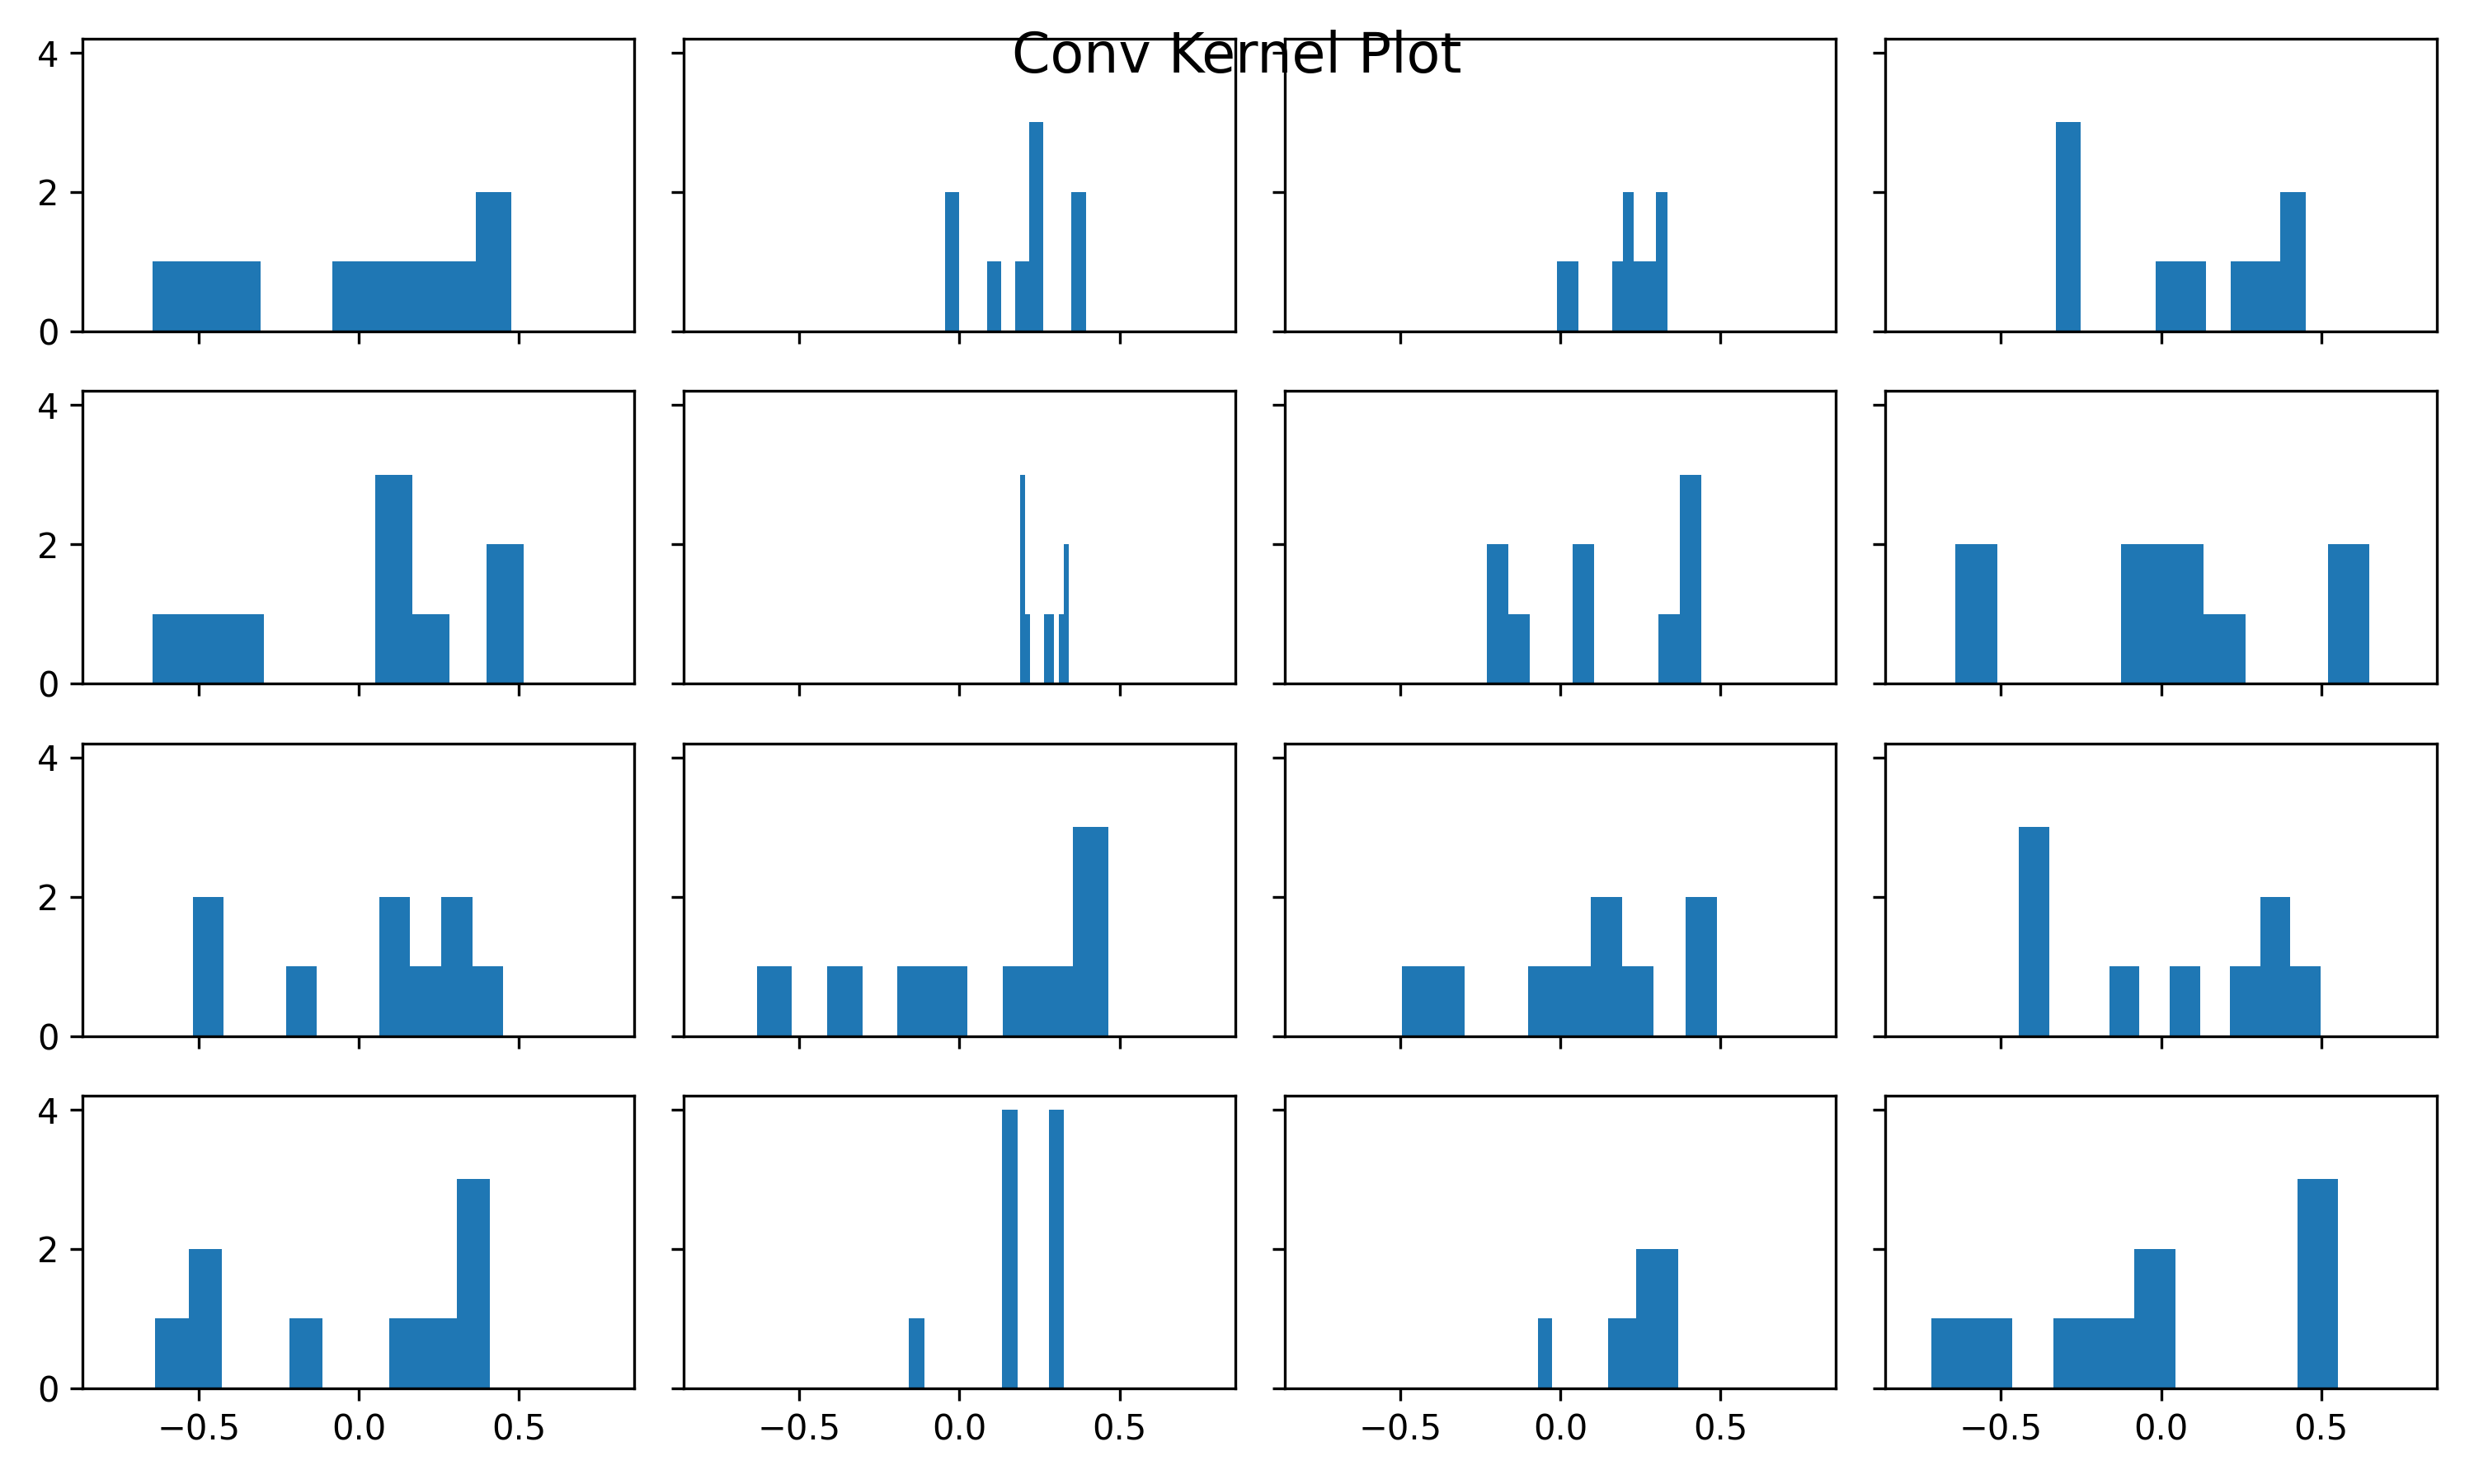
\includegraphics[height=1.6in]{../../net/images/hist_cn1_k}
        \caption{Convolutional Layer 1}
    \end{subfigure}%
    ~ 
    \begin{subfigure}[t]{0.5\textwidth}
        \centering
         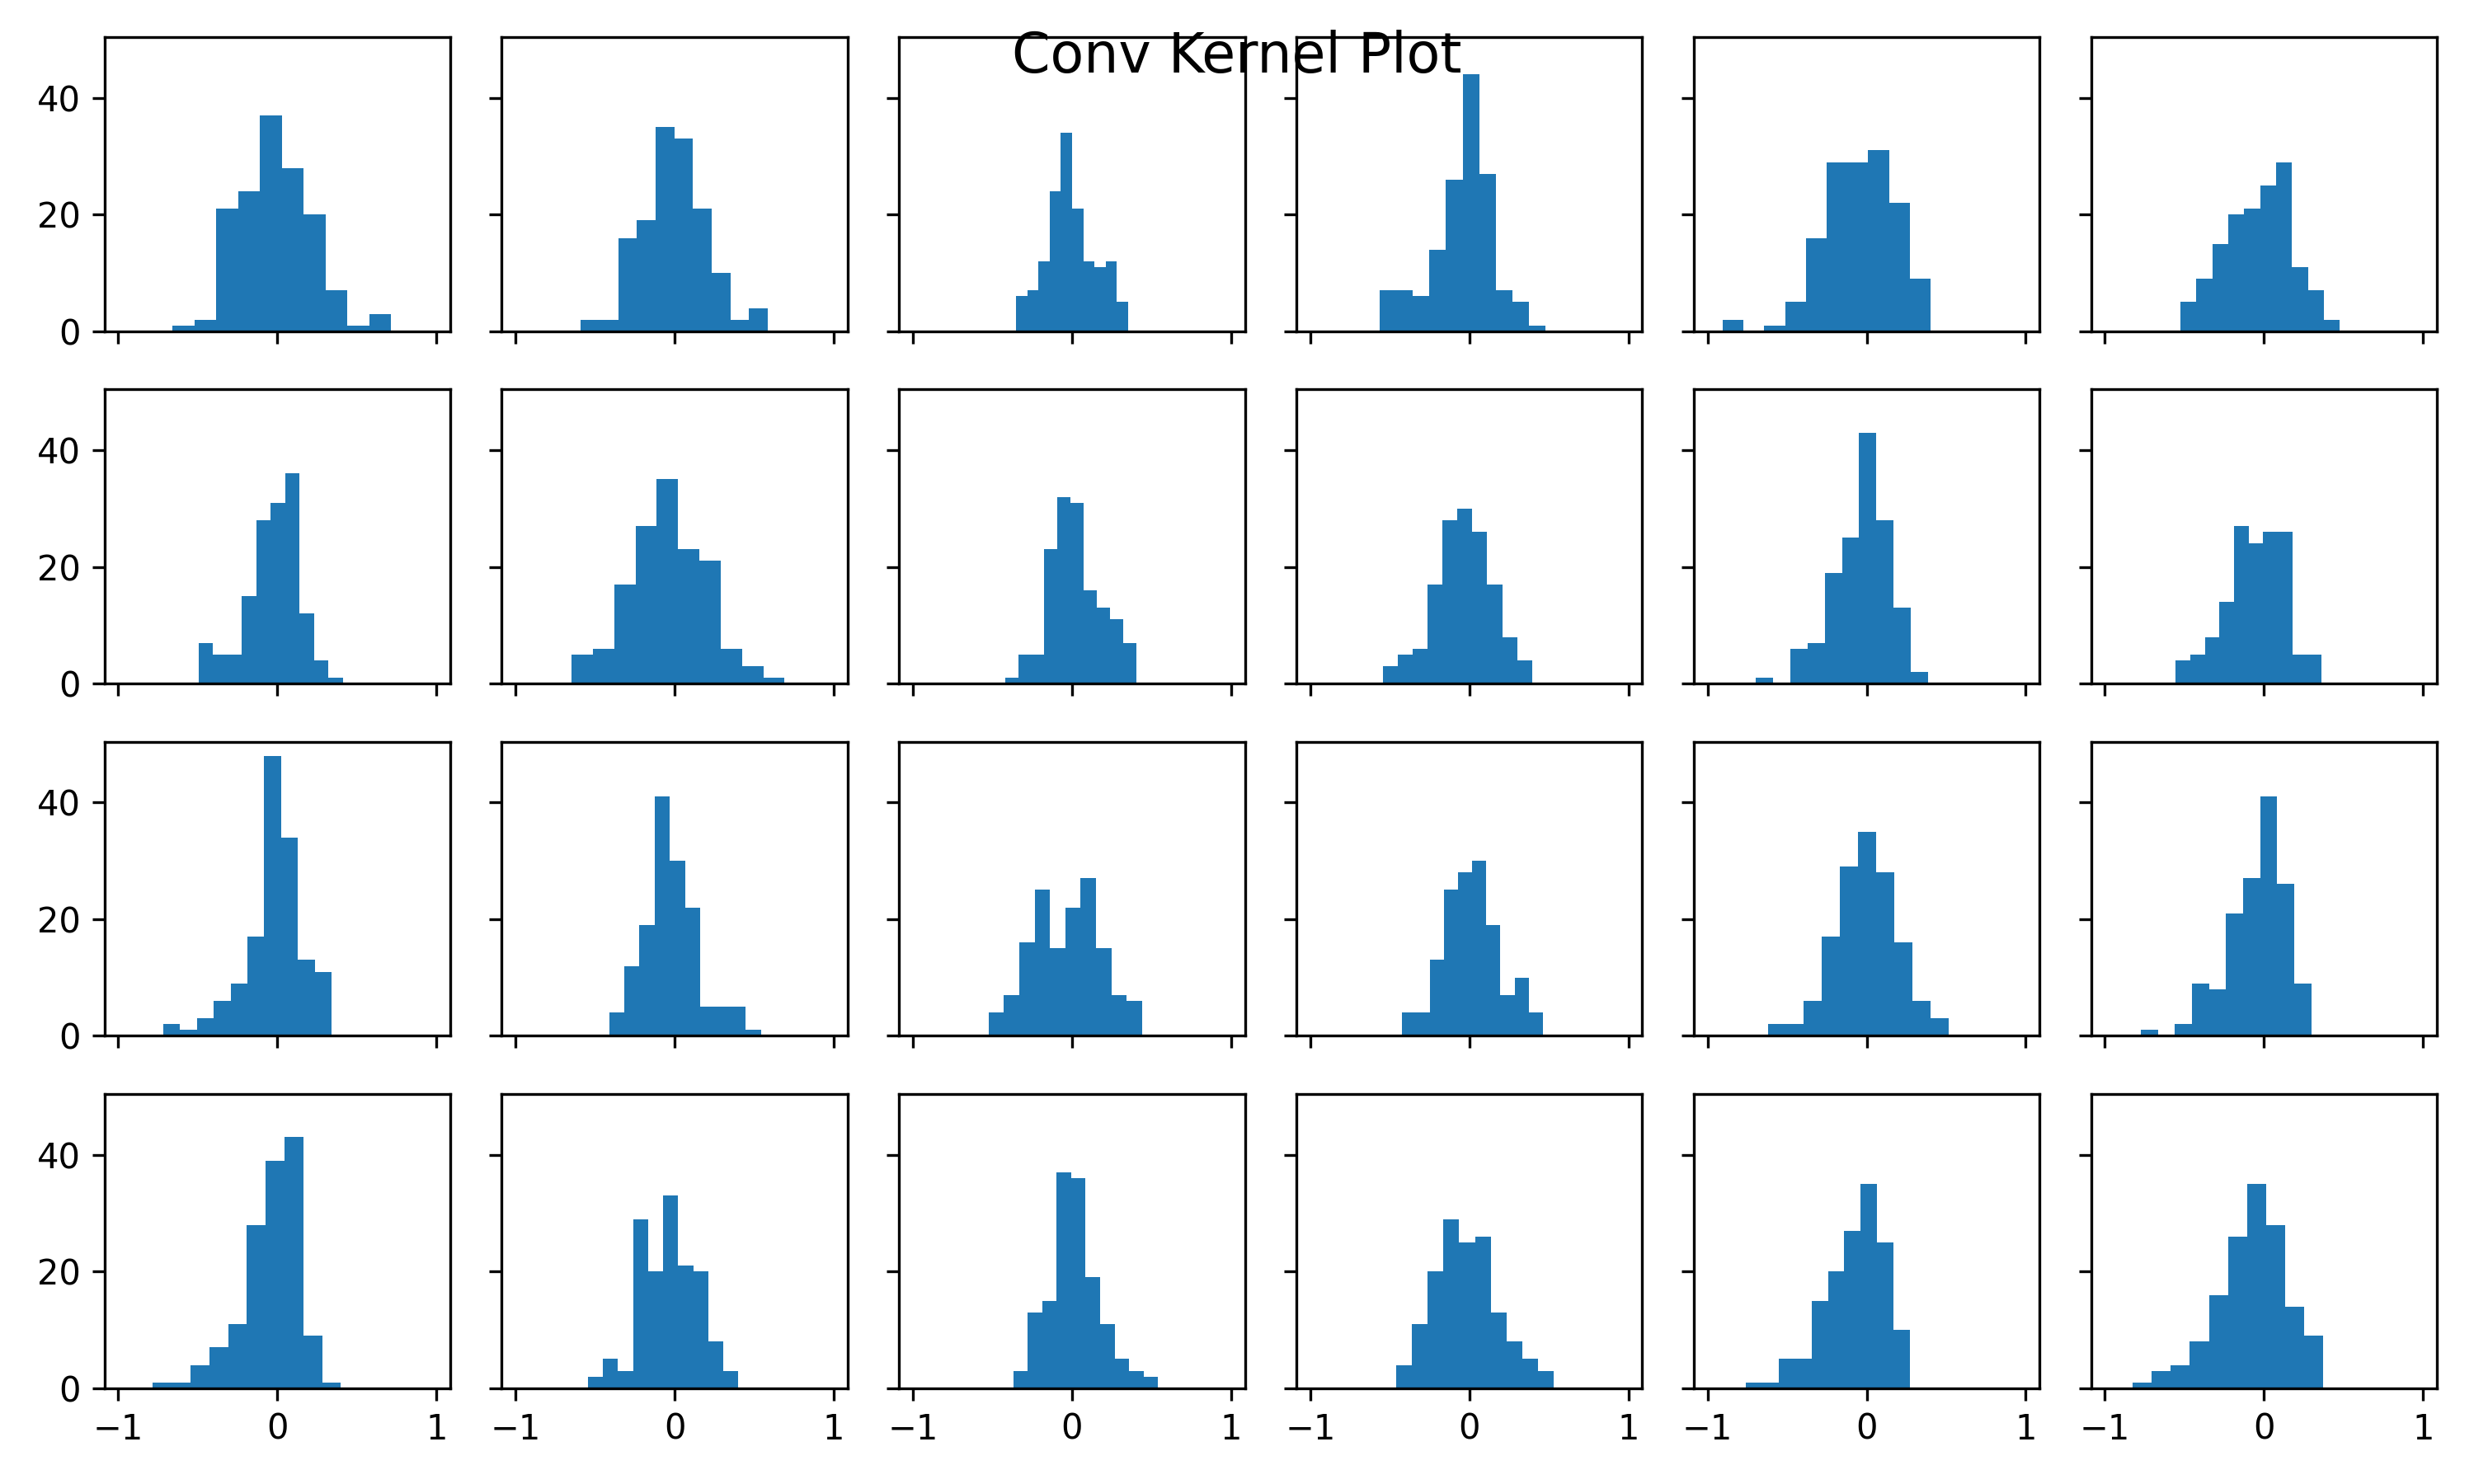
\includegraphics[height=1.6in]{../../net/images/hist_cn2_k}
        \caption{Convolutional Layer 2}
    \end{subfigure}%
    \\
    \begin{subfigure}[t]{0.5\textwidth}
        \centering
        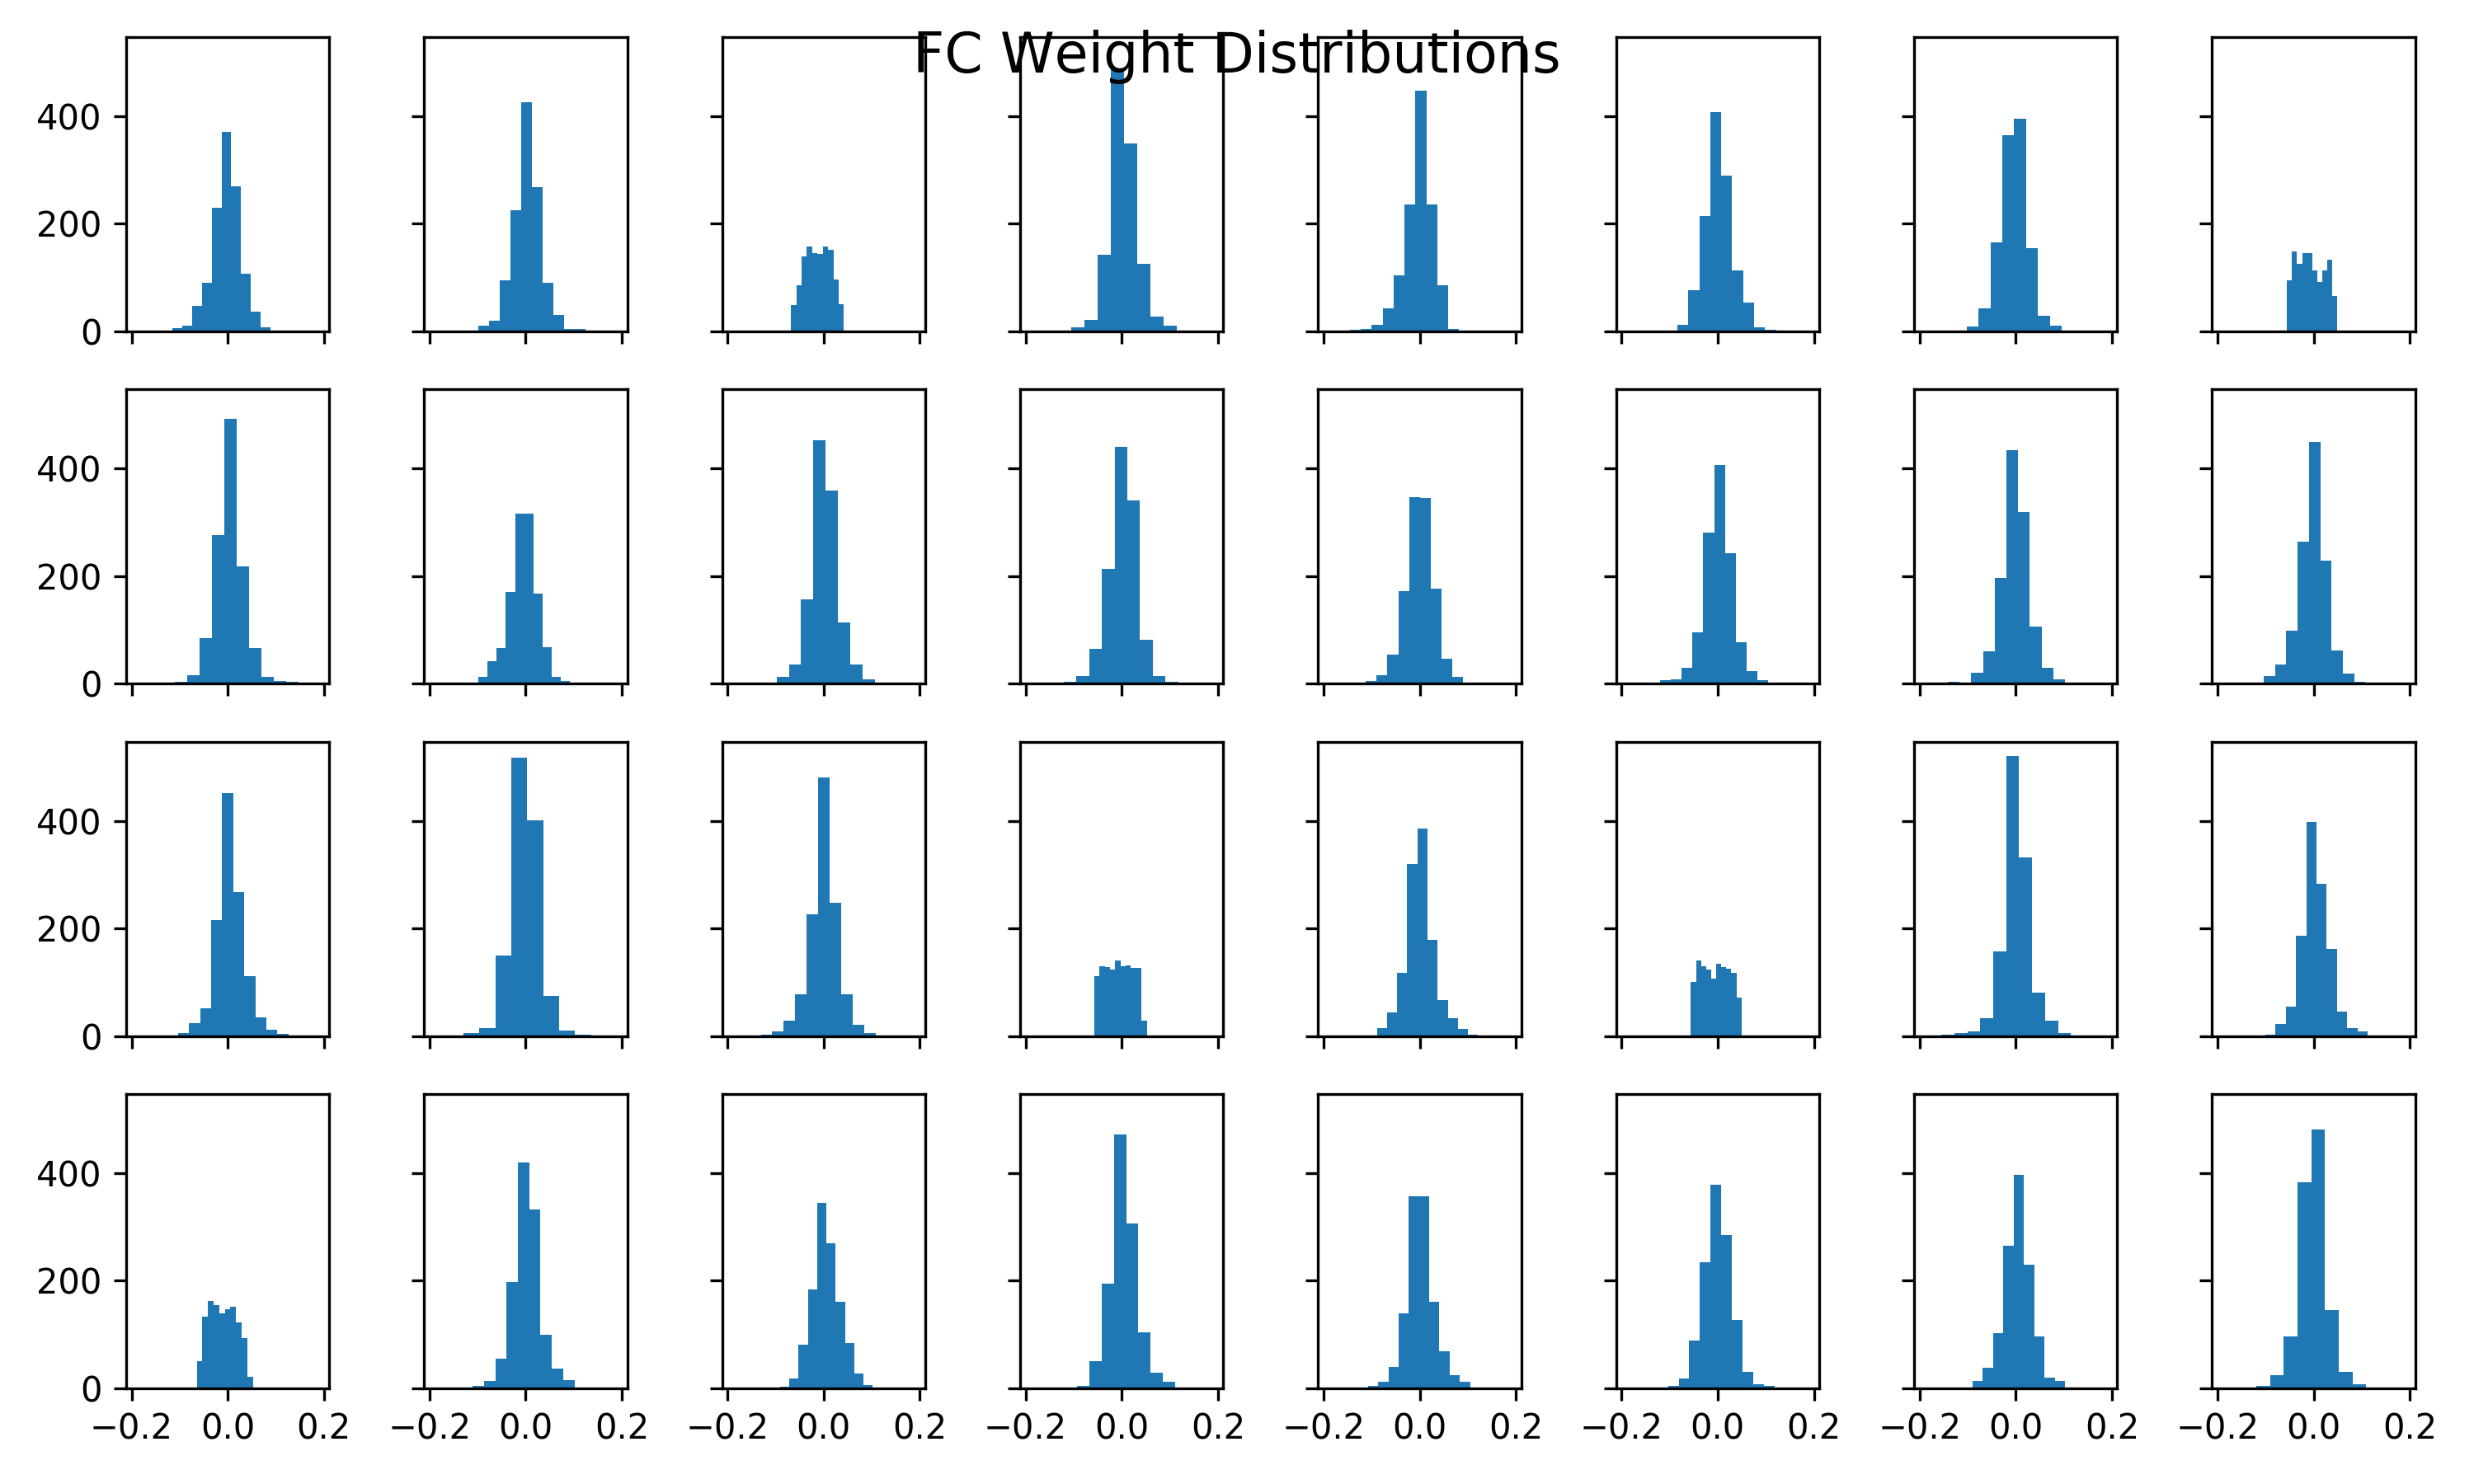
\includegraphics[height=1.6in]{../../net/images/hist_fc1_w}
        \caption{Fully Connected Layer 1}
    \end{subfigure}%
    ~ 
    \begin{subfigure}[t]{0.5\textwidth}
        \centering
         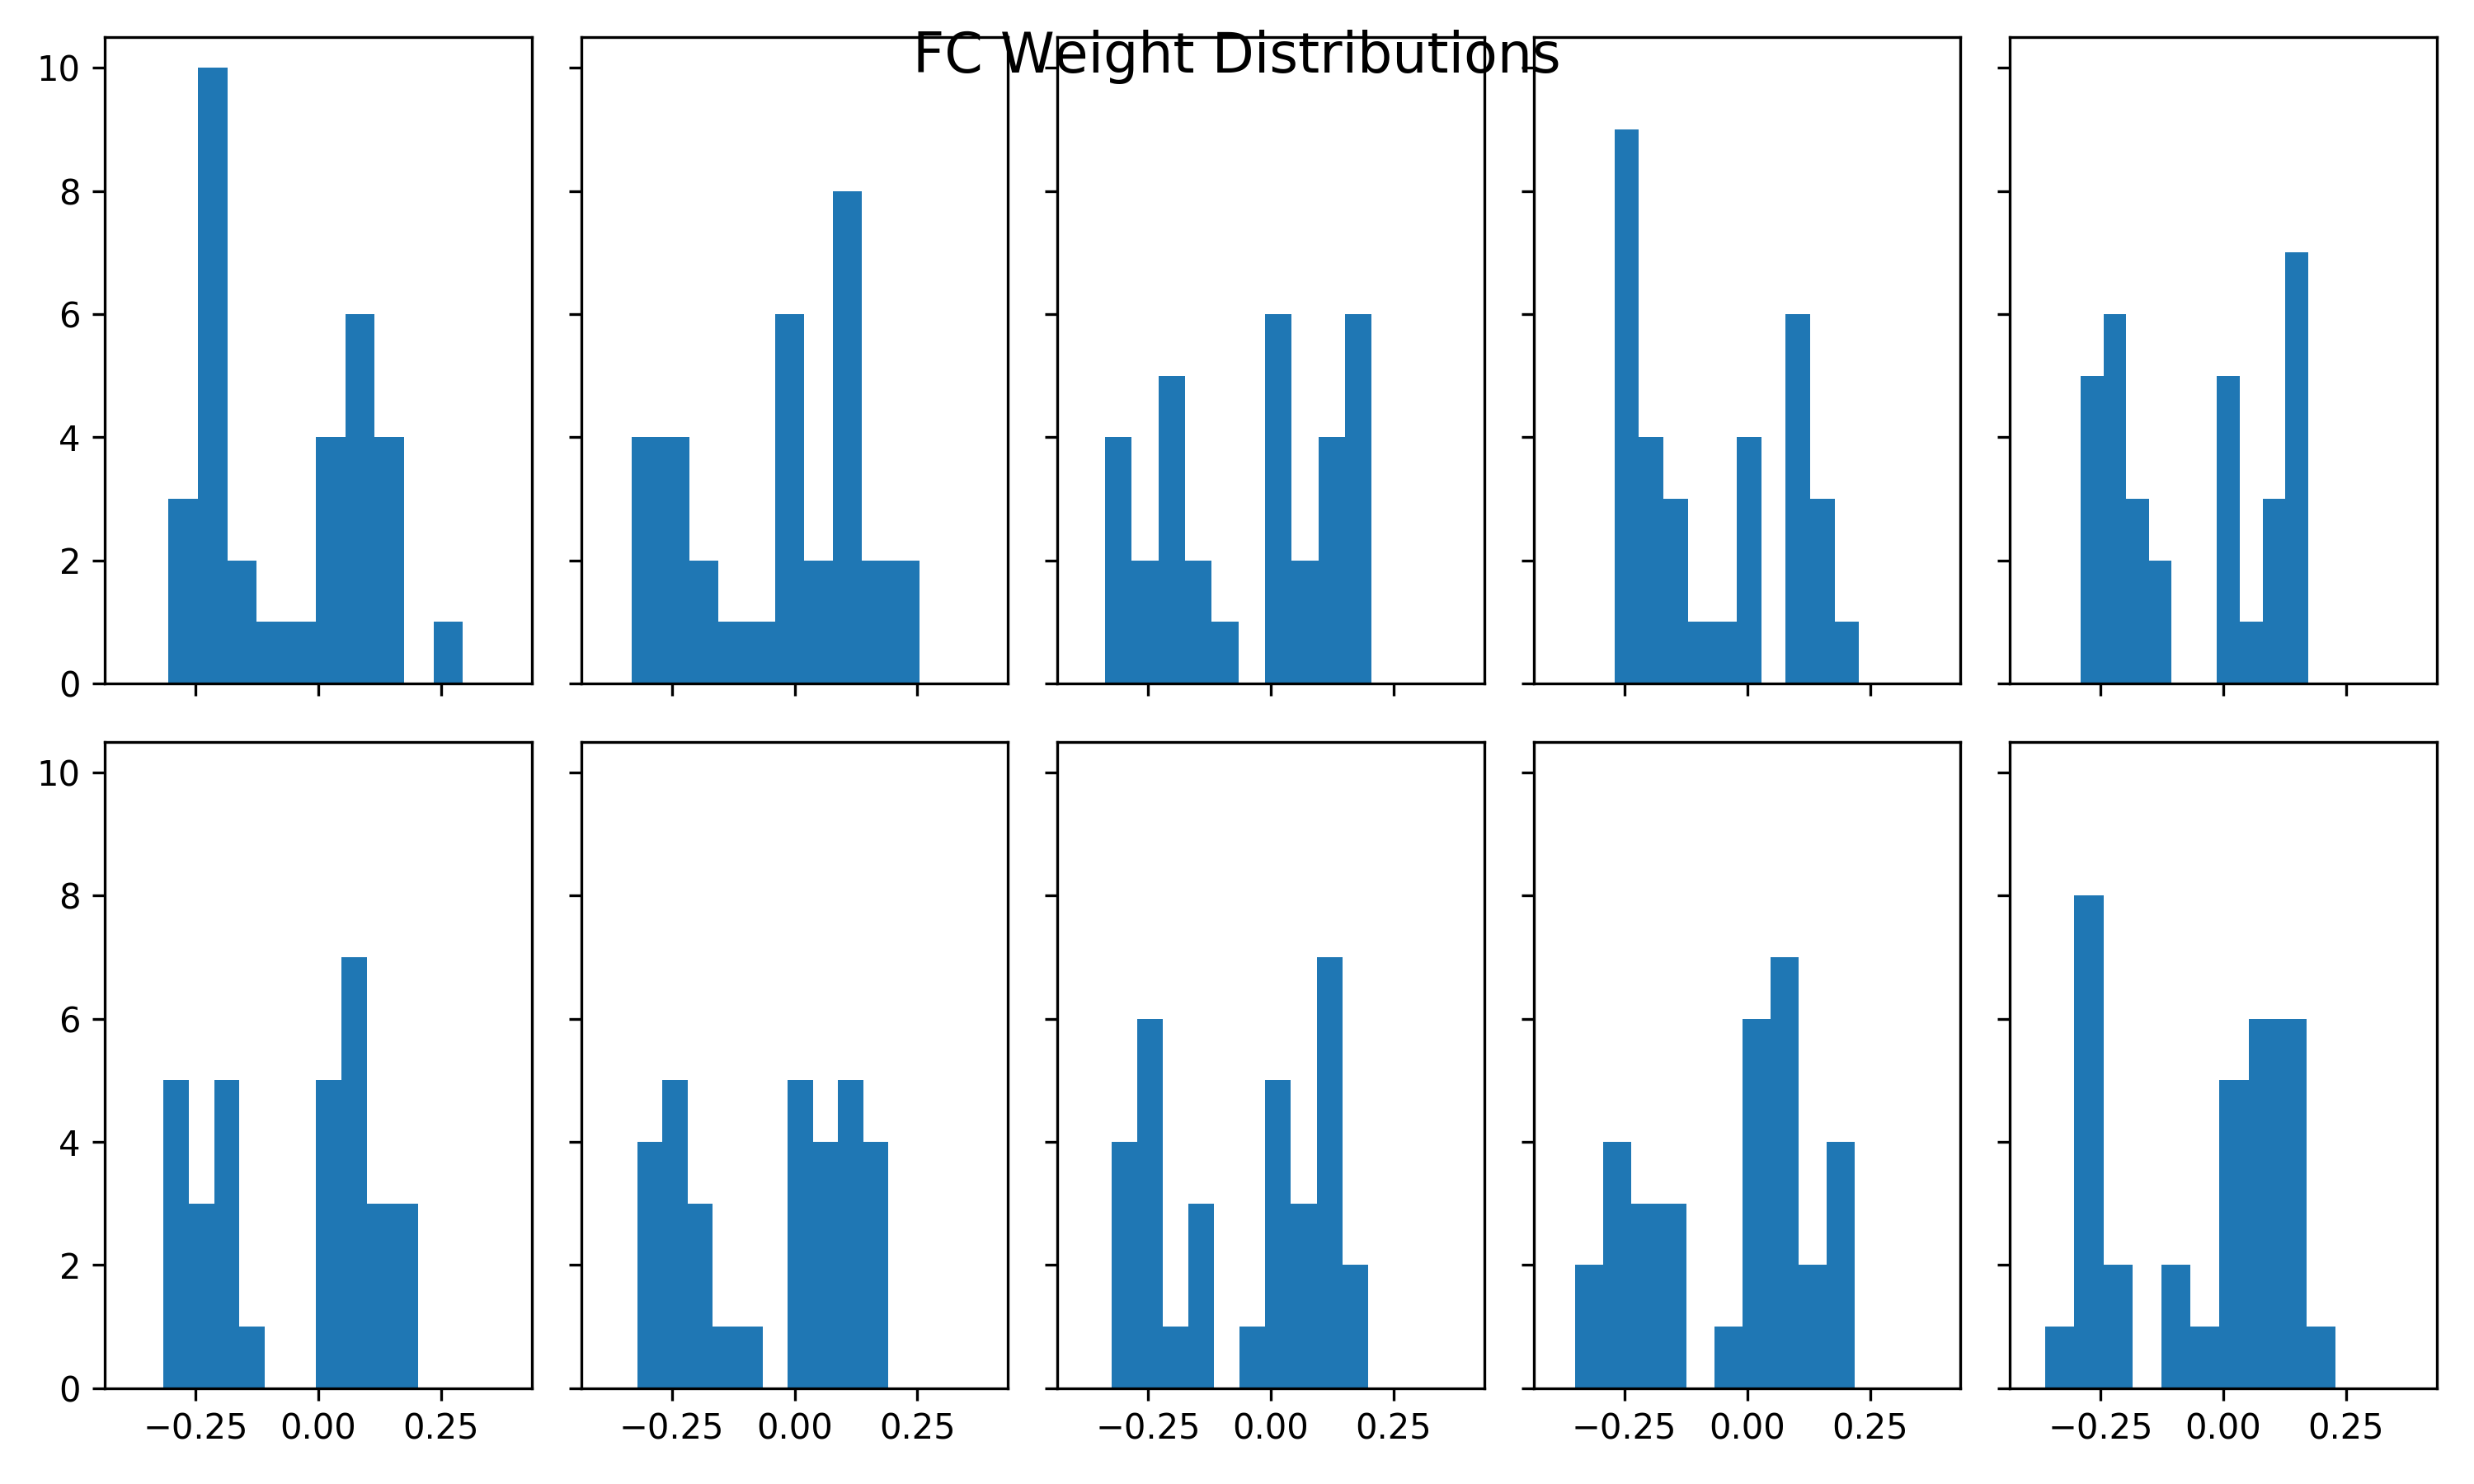
\includegraphics[height=1.6in]{../../net/images/hist_fc2_w}
        \caption{Fully Connected Layer 2}
    \end{subfigure}
    \caption{Distribution of the network weights for the different layers}
    \label{fig:network-weight-distributions}
\end{figure}

The network was reduced to fixed point integers defined by the equation
\begin{equation}
	v = Q \cdot 2 ^{-m}
\end{equation}
where both $Q$ and $m$ are integers and $v$ is the real value representation of the fixed point number. 
For our network implementation we chose a vairable fraction length for each layer and a total bitlength for $Q$ of $8$. 
This quantization can further be adjusted for each convolutional channel separately but optimization in this way were beyond the scope of this project.
The multiplication of two fixed point integers is trivial, because the product for two real values $v_1$ and $v_2$ is 
\begin{equation}
	v_1 v_2 = \text{right-shift}\left( Q_1 Q_2 \cdot 2^{-(m+m)} ; m\right)
\end{equation}
In our tests a quantization with $8$ bit fixedpoint integers and even $4$ bit integers showed only a small drop in accuracy of around $1 \%$.
\todo{Add Histogram}


